\chapter{Planificación del proyecto}
\section{Equipo}
El equipo de Octopus Data Insights está formado por cuatro personas, con perfiles multidisciplinares y complementarios:
\begin{itemize}
\item Fabio Inui: 
\item Teresa Martínez: matemática, con diez años de experiencia en investigación y docencia a nivel universitario,
ocho en construcción de modelos de valoración de derivados en empresa financiera de primer nivel, y cuatro de
gestión de fondos en una de las principales gestoras españolas.
% \item Javier Quintana: 
\item Silvia Santos: ingeniero industrial, con más de 15 años de experiencia en entornos productivos del sector industrial y 3 como consultora de Facility Management.
\end{itemize}

\section{Desarrollo temporal}

El desarrollo del proyecto se ha llevado a cabo a lo largo de varias fases:
\begin{itemize}
\item {\bf Obtención de datos}: esta primera fase se desarrolló a finales de Noviembre
de 2017, y se dividió en dos subtareas:
	\begin{itemize}
	\item La recogida de tuits se llevó a cabo a lo largo del periodo entre el 18 de Noviembre
y el 1 de Diciembre de 2017.
	\item En los días posteriores se llevó a cabo el análisis inicial de los tuits.
	\end{itemize}
\item La fase de {\bf limpieza de los tuits} se llevó a cabo entre el 8 de diciembre de 2017 y el 29 de Enero
de 2018, y se dividió en tres subtareas que llevamos a cabo en paralelo:
	\begin{itemize}
	\item Algoritmo para detección idioma
	\item Algoritmo para la detección del tema de referencia 
	\item Detección de usuarios relevantes (personas frente a empresas, bots)
	\end{itemize}
\item Construcción del {\bf modelo de ordenación de candidatos}: la fase final del proyecto se ha desarrollado a lo largo del mes de Febrero.
\item Por último, se lleva a cabo la {\bf generación de informes y presentación de resultados} de cara a la entrega del proyecto.
\end{itemize}
La redacción de la memoria	es una tarea continua, incorporando los 
resultados y desarrollos a medida que se han ido produciendo.

\begin{sidewaysfigure}
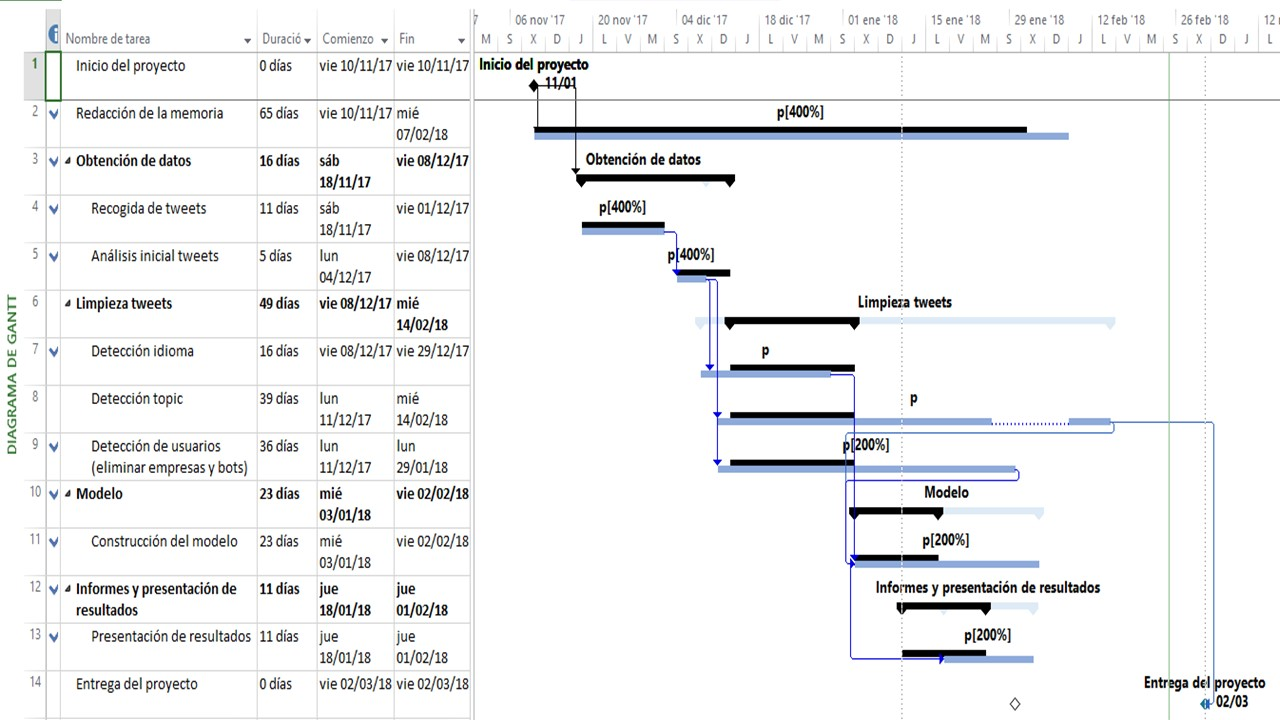
\includegraphics[width=\textwidth]{project_planning1}
\caption{Planificación del proyecto.}
\label{fig:planificacion_proyecto}
\end{sidewaysfigure}

